%%%%%%%%%%%%%%%%%%%%%%%%%%% asme2ej.tex %%%%%%%%%%%%%%%%%%%%%%%%%%%%%%%
% Template for producing ASME-format journal articles using LaTeX    %
% Written by   Harry H. Cheng, Professor and Director                %
%              Integration Engineering Laboratory                    %
%              Department of Mechanical and Aeronautical Engineering %
%              University of California                              %
%              Davis, CA 95616                                       %
%              Tel: (530) 752-5020 (office)                          %
%                   (530) 752-1028 (lab)                             %
%              Fax: (530) 752-4158                                   %
%              Email: hhcheng@ucdavis.edu                            %
%              WWW:   http://iel.ucdavis.edu/people/cheng.html       %
%              May 7, 1994                                           %
% Modified: February 16, 2001 by Harry H. Cheng                      %
% Modified: January  01, 2003 by Geoffrey R. Shiflett                %
% Use at your own risk, send complaints to /dev/null                 %
%%%%%%%%%%%%%%%%%%%%%%%%%%%%%%%%%%%%%%%%%%%%%%%%%%%%%%%%%%%%%%%%%%%%%%

%%% use twocolumn and 10pt options with the asme2ej format
\documentclass[twocolumn,10pt]{asme2ej}


\usepackage{amsthm}
\usepackage{amsmath}
% \usepackage{epsfig} %% for loading postscript figures
\usepackage{algorithm}
\usepackage{algorithmic}
\usepackage{pgfplots}
\pgfplotsset{width=7cm,compat=1.8}
\usepackage{graphicx}
\graphicspath{ {./figure/} }

\newtheorem{theorem}{Theorem}[section]
\newtheorem{lemma}[theorem]{Lemma}
\newtheorem{axiom}[theorem]{Axiom}

%% The class has several options
%  onecolumn/twocolumn - format for one or two columns per page
%  10pt/11pt/12pt - use 10, 11, or 12 point font
%  oneside/twoside - format for oneside/twosided printing
%  final/draft - format for final/draft copy
%  cleanfoot - take out copyright info in footer leave page number
%  cleanhead - take out the conference banner on the title page
%  titlepage/notitlepage - put in titlepage or leave out titlepage
%  
%% The default is oneside, onecolumn, 10pt, final


\title{Information Theory Approach to Reducing Failure Inducing Input}

%%% first author
\author{Mike Fairhurst
    \affiliation{
	Google Inc.,
    Email: mfairhurst@google.com
    }	
}

%%% second author
%%% remove the following entry for single author papers
%%% add more entries for additional authors
%%%\author{J. Michael McCarthy\thanks{Address all correspondence related to ASME style format and figures to this author.} \\
%%%    \affiliation{ Editor, Fellow of ASME\\
%%%	Journal of Mechanical Design\\
%%%        Email: jmmccart@uci.edu
%%%    }
%%%}
%%%
%%%%%% third author
%%%%%% remove the following entry for single author papers
%%%%%% add more entries for additional authors
%%%\author{Third Co-author\\
%%%        Graduate Research Assistan, Student Member of ASME\\
%%%       {\tensfb Fourth Co-author}\thanks{Address all correspondence for other issues to this author.} 
%%%    \affiliation{Title, Member of ASME\\
%%%        Department or Division Name\\
%%%        Company or College Name\\
%%%        City, State (spelled out), Zip Code\\
%%%        Country (only if not U.S.)\\
%%%        Email address (if available)
%%%    }
%%%}


\begin{document}

\maketitle    

%%%%%%%%%%%%%%%%%%%%%%%%%%%%%%%%%%%%%%%%%%%%%%%%%%%%%%%%%%%%%%%%%%%%%%
\begin{abstract}
{\it
Minimized reproductions of software issues are easier to debug. This paper
presents a new algorithm "entropy debugging" faster than the predecessor
"delta debugging". To do so, it treats the problem of crash minimization as a
set minimization/simplification problem. The fitness tests themselves on
possible subsets to consider can then be viewed as an information stream, which
lends itself well to statistical analysis and data compression techniques. This
means "entropy debugging" is likely to approach a hypothetical lower bound of
performance given an accurate statistical model of the underlying information.}
\end{abstract}

%%%%%%%%%%%%%%%%%%%%%%%%%%%%%%%%%%%%%%%%%%%%%%%%%%%%%%%%%%%%%%%%%%%%%%
%%%\begin{nomenclature}
%%%\entry{A}{You may include nomenclature here.}
%%%\entry{$\alpha$}{There are two arguments for each entry of the nomemclature environment, the symbol and the definition.}
%%%\end{nomenclature}
%%%
%%%The primary text heading is  boldface and flushed left with the left margin.  The spacing between the  text and the heading is two line spaces.
%%%
%%%%%%%%%%%%%%%%%%%%%%%%%%%%%%%%%%%%%%%%%%%%%%%%%%%%%%%%%%%%%%%%%%%%%%%%%
\section{Introduction}

Debugging a crash is easier with an example crashing input, and easiest when
that example reproduction is minimal. These inputs can be found by users,
developers, and/or tools like fuzz testing.

When these crash reproductions are not minimized, it would be ideal if there
were an algorithm that could create the minimized input. Removing one character
(or symbol of some other kind) at a time from the input is a naive algorithm
to reduce an input. If the reproduction is small and the crash reporduces
quickly, this naive algorithm works.

Delta Debugging\cite{dd} is another option. Delta Debugging resembles a binary
search where large chunks of the input are removed at a time, potentially
reducing the input greatly in few tests. However, Delta Debugging is slower than
the naive approach when the input is already close to minimal. This fits the
finding by Yu et. al that the usefulness of Delta Debugging can vary wildly in
real world scenarios\cite{ddRealPerspectives}.

Hierarchical Delta Debugging\cite{hdd} is an option for cases where the input
can be formed into a tree. Hierarchical Delta Debugging yields great results but
not all simplifications can be treated as a tree, and the time spent turning the
failure case into a tree-like structure may not be worth the improved
performance. For instance, a greybox/blackbox fuzz testing framework does not
understand the program it's fuzzing well enough to create a hierarchical
structure of the failures it finds. And malformed inputs may only crash because
the input violates the tree structure that the program expects (for instance, a
parser may crash for a particular type of mismatched parenthesis). Lastly, Yu
et. al found that both Hierarchical Delta Debugging did not yield definite
improvements over Delta Debugging in efficiency in real world
application\cite{ddRealPerspectives}.

In spite of these issues, simplification of failure cases and simplification of
fuzz corpora by code coverage measures are both still tasks performed by
frameworks and those frameworks need algorithms with good performance.

Entropy Debugging is a new algorithm presented here which aims to achieve close
to optimal average case performance for all types of inputs, by taking a
statistical/information theory approach to the problem of set simplification
over an arbitrary fitness test.

\subsection{Formalizations}

Delta Debugging\cite{dd} and the algorithm presented here are both algorithms
that solve the following general problem.

\subsubsection{Set Minimization}
We define the problem of \textbf{set minimization} as $sm(\alpha, t) = \alpha'$,
where $\alpha$ is an ordered or unordered set, $t$ is a blackbox function, and
$\alpha'$ is the smallest set $s$ such that $s \subset \alpha$ and $t(s)$.
(Zeller's "local minimum"\cite{dd}).

Given that $t$ is an abritrary black box function, its performance is unbounded.
Therefore an important measure of complexity of an algorithm performing set
minimization is the number of invocations of $t$.

Set minimization is the true goal of both Delta Debugging and the algorithm
presented in this paper, however, the complexity of $sm(\alpha, t)$ is
$2^{|\alpha|}$\cite{dd}.

Therefore a different definition is needed for practical purposes; for this
there is \textbf{n-minimality}\cite{dd}.

\subsubsection{1-minimality}

Zeller defines \textbf{n-minimality} as $min(\alpha, t, n) = \alpha'$ where
$\forall c \subset \alpha \cdot |c| - |\alpha| \leq n \Rightarrow t(c)$.
Zeller proposes that 1-minimality is the ideal target for an algorithm
approximating set minimization.

In less formal terms, n-minimality can be defined as searching for a result
where no n items in the set could be removed while still satisfying the test
function. In the case of 1-minimal, this means that no individual item in
the set can be removed on its own while satisfying $t$, though it is possible
that some pair of entries in the set (or tuples of size $n > 1$) could be.

This paper disputes the value of 1-minimality, though the algorithm presented
can help efficiently find 1-minimal results.

To do: link to disputing the value of 1-minimality

Finding a 1-minimal set is $O(n^2)$.

\subsubsection{Set Simplification}

There is also a new presented definition, which is core to the ideas presented
in this paper. We define the problem of \textbf{set simplification} as
$simplify(\alpha, t) = \alpha'$ as a subproblem of set minimization. In
simplification, it is required that $t$ satisfies
$\forall c \supset \alpha' \Rightarrow t(c)$.

\begin{theorem}
  The worst case complexity of set simplification is $O(n)$.
\end{theorem}

\begin{axiom}
  $t(\alpha' \setminus {c})$ iff $c \in \alpha'$.
\end{axiom}

\begin{axiom}
  $|\alpha'| \leq |\alpha|$.
\end{axiom}

\begin{lemma}
  $simplify(\alpha, t) = \{ c | c \in \alpha, t(\alpha \setminus {c}) \}$
\end{lemma}

%%% TODO: show that it takes *at least |alpha'| steps.

\begin{proof}
  Since set simplification can be translated to a list comprehension on
  $\alpha$, it cannot take more than $|\alpha|$ steps to find.
\end{proof}

\begin{theorem}
  The result of set simplification is also n-minimal for all n.
\end{theorem}

\begin{proof}
  Assume that $\alpha'$ is not n-minimal for some $n > 0$. That means
  $\exists c \subset \alpha' \cdot |c| - |\alpha'| > n \land t(c)$. That
  implies $|c| < |\alpha'|$. However, if $t(c)$ and $|c| < |\alpha'|$, then
  $|\alpha'|$ is not the smallest $s$ such that $t(s)$. This is a contradiction.
  Therefore if the set simplification result $\alpha'$ is n-minimal for all n.
\end{proof}

In practice, few nontrivial tests satisfy the requirements to make set
simplification applicable. However, this paper uses set simplification as a
benchmark of algorithmic performance and suggests it as a good approximation for
many use cases where set minimization is desired.

\subsection{Information Theory Approach}

The novel approach taken to find a better algorithm of approximating set
minimization is to translate test function results into an information stream.
This paper explores how that information stream can be compressed efficiently.

Expressing the problem as a data stream is easier from the lens of \textit{set
simplification} than \textit{set minimization}. (Later,
\textit{set minimization} will be compared to noisy data streams).

To do: eventually compare set minimization to noisy data streams.

From here on, this paper assumes that $\alpha$ is a \textit{totally ordered set}.

\subsubsection{Simplification as Information}

For each member $e_i \in \alpha'$, the "underlying state" can be viewed as
important ($e_i \in \alpha'$) or unimportant ($e_i \notin \alpha'$). As a 
character coding, this may look like $uuiuuiuui$. Of course, a better encoding
is a binary encoding, $001001001$.

%%% this should be formalized.
This binary encoding is has some significance. It represents the \textit{brute
force encoding} of performing set minimization on the input. In other words, if
each character is tested individually and in order for membership of $\alpha'$
(by $t(\alpha \setminus {e_i})$), the ordered results of these invocations of
$t$ will be true or false corresponding to the 0s and 1s above.

The field of information theory suggests that this stream should be encodable
in a more optimal encoding.

In the example above, one such encoding would be $0=00, 1=1$. Under this
encoding, the previous example can be compressed to $010101$, saving four bits
of information.

\subsubsection{Statistical Modeling of the Simplification Data}

Having a statistical model of the simplification data is required in order to
create an optimal encoding of that data.

The simplest statistical model of this data is merely having $p(e \in \alpha')$
for any $e \in \alpha$.

This model would not assume any correlation between the individual members of
the minimal set. While this is reasonable given than $t$ is an arbritrary
function, it does not match what is typical of real world scenarios.

The cases given by Zeller\cite{dd} exemplify this. The simplest failure inducing
inputs studied for \textit{delta debugging} typically represent contiguous
subsets of the original input.

Therefore this paper suggests markov transitions as a simple but more powerful
model. A set of markov transition probabilities (from $u$ to $i$ and $i$ to $u$)
are powerful enough to capture correlation, discorrelation, and independence
between bits in the data stream.

Now it is possible to create an optimal coding against this markov model.

\subsubsection{Optimal Markov Encoding}

Given a markov model and an input length, it is now possible to construct an
optimal encoding for the sequence using huffman coding. Where $\beta$ is the set
of all possible sequences of items $u$ and $i$,

$optimal = Huffman(\beta)$.

If we had this code, we would be able to optimally represent inputs like
$uuiuuiuui$, for any arbitrary length, given any arbitrary underlying markov
model.

Note: this is optimal \textit{if the markov model is the best statistical model}.
There may be other more accurate statistical models that lead to more optimal
encodings still.

However, this approach is not scalable, as $|\beta| = 2^{|n|}$.

\subsubsection{Simplification Chunks}

To simplify the construction of our huffman code, we must construct a smaller
set of symbols that makes progress on the whole input. One possibility is to
construct huffman codes over each "character" ($i$ and $u$) in the input. This
would merely result in the unimproved encodings ($i=0$, $u=1$ or vice versa),
regardless of the entropy of the markov model. This can be thought of as
"quantization error," where an input entropy below 1 will still yield an average
performance of at least 1 in a huffman tree.
%%% Formalize this^

There is a natural way to segment the simplification data that matches practical
observations of real world use cases for these algorithms, as well as having
this "quantization error" end up matching the worst case scenario of
simplification.

The best case performance of simplification is $O(|\alpha'|)$. It therefore is
reasonable to choose the huffman code symbol sets such that any quantization
error that results from the set having entropy less than 1, will not necessarily
decrease algorithmic worst case performance.
%%% Formalize this^

It is therefore this paper's suggestion that huffamn codes be used to encode
\textit{sequences of repeated $u$ ending in a single $i$ or end of input}, in
the style of Golomb-Rice run-length encoding\cite{golombRice}.

Here's such an encoding: $i=0$, $ui=10$, $uui=11$, $uu\epsilon=11$.

This example is of course, the identity encoding.

As an example of an improved encoding, our original example may be optimally
encoded (with ..., $uui=0$, ...), to $000$.

\subsubsection{Runnable Identity Encodings}

Unfortunately, the problem of compressing our original simplification data is
not yet done. The encodings created by huffman's algorithm are not guaranteed to
create a \textit{runnable identity encoding}.

Take the above example, where $uui=0$. This is not runnable in its indentic form.
There is no single value $v$ such that $t(v)$ iff ${uui} \in \alpha'$. Through
two tests this is possible (test that $t(\{i\}) \land \neg t(\{\}))$, however, those
two tests imply the \textit{runnable encoding} for this sequence is $10$ and not
$0$. Given that they do not share an identity, $uui=0$ is not a
\textit{runnable identity encoding}.
%%% Maybe need notation to signify t(ui) etc...

\begin{theorem}
  Huffman coding is not guaranteed to return a runnable identity encoding.
\end{theorem}

\begin{lemma}
  If $p(i)=0.25$, $p(ui)=0.5$, and $p(uui)=0.25$, $huffman(\{i, ui, uui\})$
  produces $ui=0$, $i=10$, $uui=11$.
\end{lemma}

\begin{axiom}
  If this is a runnable identity encoding, then some value $v$ exists such that
  $t(v)$ iff $ui \land \neg (i \lor uui)$.
\end{axiom}

\begin{axiom}
  $t(v) = r$, and $r$ is either $true$ or $false$.
\end{axiom}

\begin{axiom}
  $t(v)$ is false in all cases where $v \not\supset \alpha'$ $v$ and true in all
  cases where $v \supset \alpha'$.
\end{axiom}

\begin{axiom}
  $v \supset \alpha'$ or $v \not\supset \alpha'$.
\end{axiom}

\begin{axiom}
  $\alpha$ must be at least three items $\{..., a, b, c, ...\}$
\end{axiom}

\begin{axiom}
  $t(v)$ must be $r$ in the case that $b \in \alpha'$ and $a \notin \alpha'$.
\end{axiom}

\begin{axiom}
  $t(v)$ must be $\neg r$ in the case then $a \in \alpha'$.
\end{axiom}

\begin{axiom}
  $r$ may be true or false: if r is always true or always false then $t(v)$
  distinguishes nothing.
\end{axiom}

\begin{lemma}
  If $a \in v$ and $r = true$, $v \supset \alpha'$, so it is possible that
  $a \in \alpha'$ or $a \notin \alpha'$. Since $r = true$ distinguishes between
  $b \in \alpha'$ or $a \notin \alpha'$, it must be that $a \notin v$.
\end{lemma}

\begin{lemma}
  Since $a \notin v$, $r = true$ implies that $a \notin \alpha'$. Therefore
  whenever $r = true$ it must also be true that $b \in \alpha'$ in all cases.
\end{lemma}

\begin{lemma}
  When $b \in \alpha'$ and $r = true$, then $v \supset \alpha'$, and therefore
  also $b \in v$.
\end{lemma}

\begin{proof}
  When $b \in v$ and $v \supset \alpha'$ and $b \notin \alpha'$, $r = true$,
  which is a contradiction.
\end{proof}
%%% ^ this could *surely* be cleaned up.

Constructing a runnable identity encoding requires constructing a decision tree
in which every branch in the tree (or bit in the encoding) corresponds to a
single invocation of $t$ for some derivable input $v$.

For the sequence encoding described here, this is equivalent to an
\textit{ordered tree} (that is to say, a tree whose leaves maintain a known
ordering).

There is a very simple ordering that ensures a
\textit{runnable identity encoding}: given two symbols $a$ and $b$, we say 
$a < b$ iff $|\{u | e \in a, e = u\}| < |\{u | e \in b, e = u\}|$ (that is, the
symbols are ordered in terms of how many unimportant characters that symbol
finds).

\begin{theorem}
  An ordered tree over this relation is a \textit{runnable identity encoding}.
\end{theorem}

\begin{lemma}
  Let our symbol set be $i$, $ui$, $uui$, $u..._ni$.
\end{lemma}

\begin{lemma}
  There is some root of the tree $r = Branch(r', r'')$. Since the tree is
  ordered, all symbols in $r'$ are $i$, $ui$, $uui$, ... $uuu..._ji$ for some $j$,
  and all symbols in $r''$ are $uuu..._{j+1}i$, $uuu..._{j+2}i$, $uuu..._ni$.
\end{lemma}

\begin{lemma}
  $uuu..._ei$ "describes" $\alpha'$ when $\alpha[e + 1 + c] \in \alpha'$ (where
  $c$ is the offset of the encoder in the data stream), and
  $\forall w \leq e > 0 \rightarrow \alpha[w + c] \notin \alpha'$.
\end{lemma}

\begin{lemma}
  There is some value $v$ such that $t(v)$ is true for all possible $\alpha'$
  such that $uuu..._{j+q}i$ "describes" $\alpha'$ where $q > 0$. Additionally,
  for that value $v$, $t(v)$ is false for all $u..._{j+q}i$ where $q \leq 0$.
  (Note that this implies the tree searches \textit{rightwards} on $true$).
\end{lemma}

\begin{lemma}
  Assume $v$ is the smallest superset of all sets that are "described by"
  $uuu..._{j+q}i$" for all $q > 0$. Since $\alpha[j + q + 1 + c] \in \alpha'$,
  then $\forall e > j + q + c \rightarrow e \in \alpha'$. Since $t(v)$ is true
  and $t(x) = x \supset \alpha'$, it holds that
  $\forall e > j + q + c \rightarrow e \in v$.
\end{lemma}

\begin{lemma}
  Assume that $\forall e \leq j + q + c \rightarrow e \notin v$. In this case,
  $v$ is not a superset of any set "described by" any $uuu...{j-1}$. Therefore,
  the there is some value $v$ that bisects all symbols in one invocation of $t$.
  (Once again, note that this implies \textit{rightwards} traversal on $true$).
\end{lemma}

\begin{proof}
  Since a value $v$ exists which bisects the symbol set $i$, $ui$, $uui$, ...
  $uuu..._ji$, $uuu..._{j+1}i$, ... $uuu..._ni$ for any $j$ given $t(v)$, this
  problem is functionally equivalent to any ordered decision tree on integers
  using $>$, and the resulting tree will be equivalent to a
  \textit{runnable identity encoding}.
\end{proof}

\subsubsection{Optimal ordered decision trees}

Much like huffman code, there must be an optimal ordered decision tree. The
optimal ordered tree is the tree that has the lowest possible cost as defined by

$$ cost(t) = \sum_{leaves of t} p(x) depth(x)$$

A naive algorithm to brute force the lowest cost tree is

\begin{algorithm}
  \caption{Naively build optimal ordered decision tree}
  \begin{algorithmic}
    \IF{$|items| = 1$}
      \RETURN $items[0]$
    \ELSIF{$|items| = 2$}
      \RETURN $Branch(items[0], items[1])$
    \ENDIF
    \STATE $result \leftarrow null$
    \STATE $left \leftarrow items[0]$
    \STATE $right \leftarrow items[1...]$
    \WHILE{$|right| > 0$}
      \STATE $candidate \leftarrow Branch(optimal(left), optimal(right)))$
      \IF{$result = null$ or $cost(candidate) < cost(result)$}
        \STATE $result \leftarrow candidate$
      \ENDIF
      \STATE $left \leftarrow left + right[0]$
      \STATE $right \leftarrow right[1...]$
    \ENDWHILE
    \RETURN $result$
  \end{algorithmic}
\end{algorithm}

This algorithm is not scalable, as it takes $O(n!)$ steps to complete. Howver,
for small trees it is suitable for use and guarantees minimal tests.

\subsubsection{Ordered huffman coding}

The following is a variant of huffman coding which completes in $O(n^2)$.
However, does not produce optimal trees.

Like standard huffman code, this algorithm finds the smallest pair and creates
a branch. However, unlike standard huffman code, this algorithm ensures that the
order is maintained by finding the smallest \textit{adjacent} pair. Similarly,
while standard huffman code sorts the new set of items \& branches on each
iteration, this variant will put the branch into the tree in place.

\begin{algorithm}
  \caption{Ordered huffman code}
  \begin{algorithmic}
    \LOOP
      \IF{$|items| = 1$}
        \RETURN $items[0]$
      \ELSIF{$|items| = 2$}
        \RETURN $Branch(items[0], items[1])$
      \ENDIF
      \STATE $pSmallest \leftarrow null$
      \STATE $iSmallest \leftarrow null$
      \FOR{$i \leftarrow 0$ to $|items| - 1$}
        \STATE $pCandidate \leftarrow p(items[i]) + p(items[i+1])$
        \IF{$pSmallest = null$ or $pCandidate < pSmallest$}
          \STATE $iSmallest \leftarrow i$
          \STATE $pSmallest \leftarrow pCandidate$
        \ENDIF
      \ENDFOR
      \STATE $b \leftarrow Branch(items[iSmallest], items[iSmallest + 1])$
      \STATE $items \leftarrow items[0...iSmallest] + b + items[iSmallest + 2...]$
    \ENDLOOP
  \end{algorithmic}
\end{algorithm}

In profiling, ordered huffman coding tended to produce close to optimal trees.
%%% Measure this? Define this limit?

\subsubsection{Information Gain Coding}

A common machine learning approach to generating decision trees is to split the
data set recursively on maximum information gain\cite{informationGain}.
Information gain $IG(Y, X)$ is the reduction of entropy $H(Y)$ given new
information.

$$IG(Y, X) = H(Y) - H(Y, X)$$
$$H(Y, X) = \sum_{x \in X, y \in Y} -p(x, y) log_2 \frac{p(x, y)}{p(x)}$$

Since this is an ordered tree, a decision $X$ has outcomes $\{y < n, y >= n\}$.
In this case, join probabilities easily simplify. $p(y < n, y)$ corresponds to
$p(y)$ if $y < n$, $p(y >= n, y)$ is $p(y)$ if $i >= n$, and $p(x', y)$ for all
other $x'$ is $0$.

Therefore it is possible to reduce $H(Y, X)$ in this case, given test decision
$n$, to

\begin{equation}
  \begin{aligned}
  H'(Y, n) & = \sum_{y \in Y \le n} -p(y) log_2 \frac{p(y)}{\sum_{y' \in Y \le n} p(y')}\\
           & + \sum_{y \in Y \geq n} -p(y) log_2 \frac{p(y)}{\sum_{y' \in Y \geq n} p(y')}
  \end{aligned}
\end{equation}

and can easily accomodate upper and lower bounds beyond this. Therefore it is
possible to generate an information gain decision tree with the following
algorithm.

\begin{algorithm}
  \caption{Information Gain Ordered Decision Tree}
  \begin{algorithmic}
    \STATE $pSubset(items') = \sum_{item \in items'} p(item)$
    \STATE $hSubset(items') = \sum_{item \in items'} -p(item) log_2 \frac{p(item)}{pSubset(items')}$
    \IF{$|items| = 1$}
      \RETURN $items[0]$
    \ELSIF{$|items| = 2$}
      \RETURN $Branch(items[0], items[1])$
    \ENDIF
    \STATE $hAll \leftarrow hSubset(items)$
    \STATE $maxIg \leftarrow null$
    \STATE $maxIgIndex \leftarrow null$
    \FOR{$i \leftarrow 0$ to $|items| - 1$}
      \STATE $hLeft \leftarrow hSubset(items[...i])$
      \STATE $hRight \leftarrow hSubset(items[i + 1...])$
      \STATE $ig \leftarrow hAll - hLeft - hRight$
      \IF{$maxIg = null$ or $ig > maxIg$}
        \STATE $maxIg \leftarrow ig$
        \STATE $maxIgIndex \leftarrow i$
      \ENDIF
    \ENDFOR
    \STATE $left \leftarrow igTree(items[...maxIgIndex])$
    \STATE $right \leftarrow igTree(items[maxIgIndex + 1...])$
    \RETURN $Branch(left, right)$
  \end{algorithmic}
\end{algorithm}

Information gain seems to yield slightly better results than ordered huffman
coding, however, it is slower. Therefore huffman coding is primarily used in
Entropy Debugging.

\subsubsection{Other forms of coding}

Other lossless compression schemes exist which can outperform huffman code, for
example, arithmetic coding and ANS. However, a general statement could be made
that these algorithms outperform huffman code by dealing with information in an
even more abstract manner than huffman codes. However, a \textit{runnable
identity encoding} must deal with that information concretely. Therefore these
were not applied to Entropy Debugging, but there may be room to improve Entropy
Debugging by attempting to do so.

\section{Entropy debugging}

Entropy debugging runs in three stages: presampling, adaptive consumption, and
then minimization.

\subsection{Presampling}

First, entropy debugging will presample the input to generate a basic markov
model.

It is unclear what the perfect number of presamples is. If the presampling
count is high, this prevents later stages from making large gains in few tests.
However, the presampling stage is the only stage that has true statistical
randomness. The current default hyperparameter value is to do five presamples.

Five random pairs of entries in the input are selected, and individually
checked for removability against the input function. Those that may be removed
while still satisfying the input function have their subsequent neighbor checked
as well.

Bayesian inference is used to infer the underlying $p(u_n)$ and
$p(u_n | u_{n-1})$. The base probability distribution is found via the Laplace
Rule of Succession, so if $n$ evenst are observed out of $s$ trials, the
inferred underlying probability of the next event is $\frac{n + 1}{s + 2}$.

\begin{algorithm}
  \caption{Presample}
  \begin{algorithmic}
    \STATE $choices \leftarrow$ choose $n$ random entries from $items$.
    \STATE $successes_u \leftarrow 0$
    \STATE $successes_{uu} \leftarrow 0$
    \STATE $trials_u \leftarrow n$
    \STATE $trials_{uu} \leftarrow 0$
    \FOR{$choice \leftarrow choices$}
      \IF{$t(items - choice)$}
        \STATE $successes_u++$
        \STATE remove $item$ from $items$
        \STATE $next \leftarrow$ the entry in $items$ following $item$
        \STATE $trials_{u}++$
        \STATE $trials_{uu}++$
        \IF{$t(items - next)$}
          \STATE $successes_{u}++$
          \STATE $successes_{uu}++$
          \STATE remove $next$ from $items$
        \ENDIF
      \ENDIF
    \ENDFOR
    \STATE $p_u \leftarrow (succeses_u + 1) / (trials_u + 2)$
    \STATE $p_{uu} \leftarrow (succeses_{uu} + 1) / (trials_{uu} + 2)$
  \end{algorithmic}
\end{algorithm}

With these data on probabilities, we infer $p(u)$ and $p(uu)$. We may then infer
$p(i)$, $p(ii)$, $p(iu)$, and $p(ui)$.

\begin{eqnarray}
  p(i) & = & 1 - p(u) \\
  p(ui) & = & 1 - p(uu) \\
  p(iu) & = & 1 - p(ii)
\end{eqnarray}

This trivially covers all but $p(ii)$, which may also be inferred with slightly
more work:

\begin{equation}
  \begin{aligned}
    p(ii) & p(i) + p(u) p(ui) & = & p(i) \\
    p(ii) & p(i)              & = & p(i) - p(u) p(ui) \\
    p(ii) &                   & = & \frac{p(i) - p(u) p(ui)}{p(i)}
  \end{aligned}
\end{equation}

It is now possible to estimate the probabilty of any sequence, with or without
a preceeding state.

\subsection{Adaptive Consumption}

The adaptive consumption stage of Entropy Debugging sweeps the input from left
to right, forming decision trees which are walked to find an outcome. That
outcome is read to reduce the input, and update the markov model.

The symbol set and tree size is capped, though the following algorithm writeup
elides that detail. When the tree is capped, a symbol $uuuu..._n$ may be built,
which requires slight offset \& probability adjustments to be correct, but
otherwise does not significantly deviate from what's written below. By capping
symbol and tree size, extremely large and sparse inputs may be less optimally
solved, however, it reduces pathological cases that may lead to $O(n^3)$
complexity. In Entropy Debugging, tree size caps are hyperparameters. The
default values are to cap the tree to 1000 symbols, where each symbol has at
least a 30\% probability.

Trees may be built with any algorithm. This behavior may be customized as a
hyperparameter. The default behavior is to build optimal trees for symbol sets
of length 10 or less, huffman-like trees for symbol sets of length 51 or
greater, and between that, a combinator of information gain, optimal, and
huffman like is used: trees of size six or less are built optimally, and for
other trees, both huffman and information gain trees are built, of which the
lowest cost tree is used (and this process recurses).

\begin{algorithm}
  \caption{Adaptive consume}
  \begin{algorithmic}
    \STATE $state \leftarrow "unknown"$
    \FOR{$i \leftarrow 0 to |items|$}
      \STATE $symbols \leftarrow \{uuu..._ni | n \in \{0, 1, ...|items|\}\}$
      \STATE $p_{first} \leftarrow \{p(i | state)\}$
      \STATE $p_{rest} \leftarrow \{p(u | state) * p(uu) ^ (n - 1) * p(ui) | n \in \{1, 2, ...|items|\}\}$
      \STATE $symbols_p \leftarrow p_{first} + p_{rest}$
      \STATE $tree \leftarrow buildTree(symbols, symbols_p)$

      \WHILE{$tree$ is a branch}
        \STATE $pivot \leftarrow$ rightmost leaf of the left branch of $tree)$
        \STATE $candidate \leftarrow items[...i, i + |pivot|...]$
        \IF{$test(candidate)$}
          \STATE $tree \leftarrow $ right branch of $tree$
        \ELSE
          \STATE $tree \leftarrow $ left branch of $tree$
        \ENDIF
      \ENDWHILE

      \STATE $outcome \leftarrow tree$
      \STATE $items \leftarrow items[...i, i + |outcome| - 1...]$
      \STATE $successes_u \leftarrow successes_u + |outcome| - 1$
      \STATE $trials_u \leftarrow trials_u + |outcome|$
      \STATE $successes_{uu} \leftarrow successes_{uu} + |outcome| - 2$
      \STATE $trials_{uu} \leftarrow trials_u + |outcome| - 3$
      \STATE $state \leftarrow $ final state in $tree$
    \ENDFOR
  \end{algorithmic}
\end{algorithm}

Note that these updates to the markov model contain sampling bias. In
benchmarks, performance is still good. A reasonable explanation is that some
sampling bias is a good thing, as it allows the algorithm to adapt somewhat to
local variations in the distribution.

The algorithm can be run without adjusting the markov model. This is reasonable
if a statistical model for a corpus has already been built.

\subsection{Minimization}

The final stage of entropy debugging is the minimization phase. It is optional
in our algorithm. At this point, the problem of \textit{set simplification} is
solved, however, the minimization phase provides \textit{set minimization}.

In tests, this phase can behave somewhat pathologically, which is to be expected
since it is $O(n^2)$ complexity instead of linear time.

The process is a very simple character by character sweep until a pass completes
making no progress.

The reason why this phase is so naive is simple.

Consider the alternative case where entropy debugging is performed iteratively
until entropy debugging makes no progress. For a low entropy input, entropy
debugging will outperform a brute force search. However, for a high or medium
entropy input, there is no way to beat a brute force search, and therefore
entropy debugging will revert to that approach automatically.

A minimized input is almost by definition a high entropy input. Aside from
pathological cases (not seen in any experiment done for this paper), it holds
that it is simpler and faster to merely choose a brute force approach
immediately.

See discussions on the value of minimization over simplification.

\section{Results}

\subsection{Delta Debugging Case Studies}

Zeller\cite{dd} included some case studies in the original publication of
Delta Debugging which have been reproduced. Two are related to a gcc bug, and
one is a crash in firefox when printing a $<SELECT>$ tag. These offer a good
starting point of comparison to Entropy Debugging.

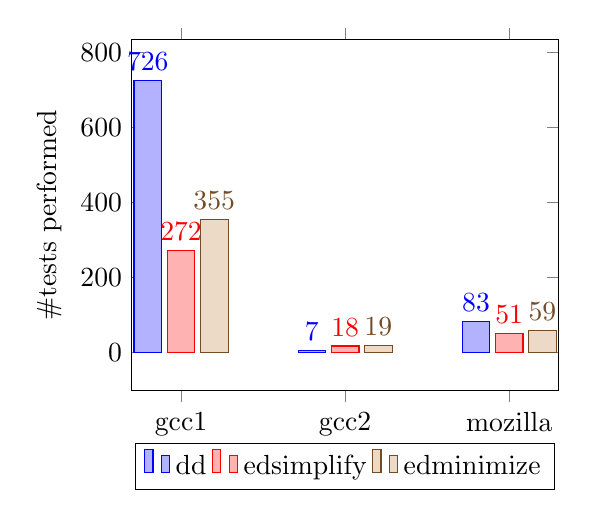
\begin{tikzpicture}
\begin{axis}[
    ybar,
    enlargelimits=0.15,
    legend style={at={(0.5,-0.15)},
      anchor=north,legend columns=-1},
    ylabel={\#tests performed},
    symbolic x coords={gcc1,gcc2,mozilla},
    xtick=data,
    nodes near coords,
    nodes near coords align={vertical},
    ]
\addplot coordinates {(gcc1,726) (gcc2,7) (mozilla,83)};
\addplot coordinates {(gcc1,272) (gcc2,18) (mozilla,51)};
\addplot coordinates {(gcc1,355) (gcc2,19) (mozilla,59)};
\legend{dd,edsimplify,edminimize}
\end{axis}
\end{tikzpicture}

As shown above, entropy debugging is able to minimize the first gcc crash input
in 52\% faster than delta debugging -- it is also able to simplify it in 37\% of
the time. Similarly, entropy debugging is 29\% faster at minimizing the mozilla
crash input, and can simplify it in 61\% of the time.

For the second gcc crash, entropy debugging takes nearly twice as long. Why?
The difference comes down to assumptions made by the algorithms. The input
contains 30 items, and the minimal subset is a single item. Delta Debugging
assumes this sort of input is likely, and the search it performs works out to be
a perfect binary search. On the other hand, Entropy Debugging assumes nothing
about the underlying information. It takes 10 checks just to presample the input
(with default hyperparameters), already losing to Delta Debugging. It then
executes 8 checks to simplify or 9 checks to minimize the input, which is
slightly behind Delta Debugging. In essence, the difference is the assumptions
made by the algorithms, combined with the small size of the input.

It is possible, in circumstances like this, to run entropy debugging without any
presampling, and to seed a custom starting probability distribution. In this
case, the second gcc crash input can be simplified by entropy debugging in six
checks. In general, this is not necesary, as Entropy Debugging beats
Delta Debugging for a very large range of markov model probabilities.

\subsection{Generated Data}

To more directly measure the point at which Delta Debugging may perform better,
than Entropy Debugging, generated data from various markov models are fed into
both algorithms and compared below. In addition, a naive brute force is plotted.
Delta Debugging often exceeds the naive approach by nearly 3x, while Entropy
Debugging fits itself to the curve.

\begin{figure}
  \centerline{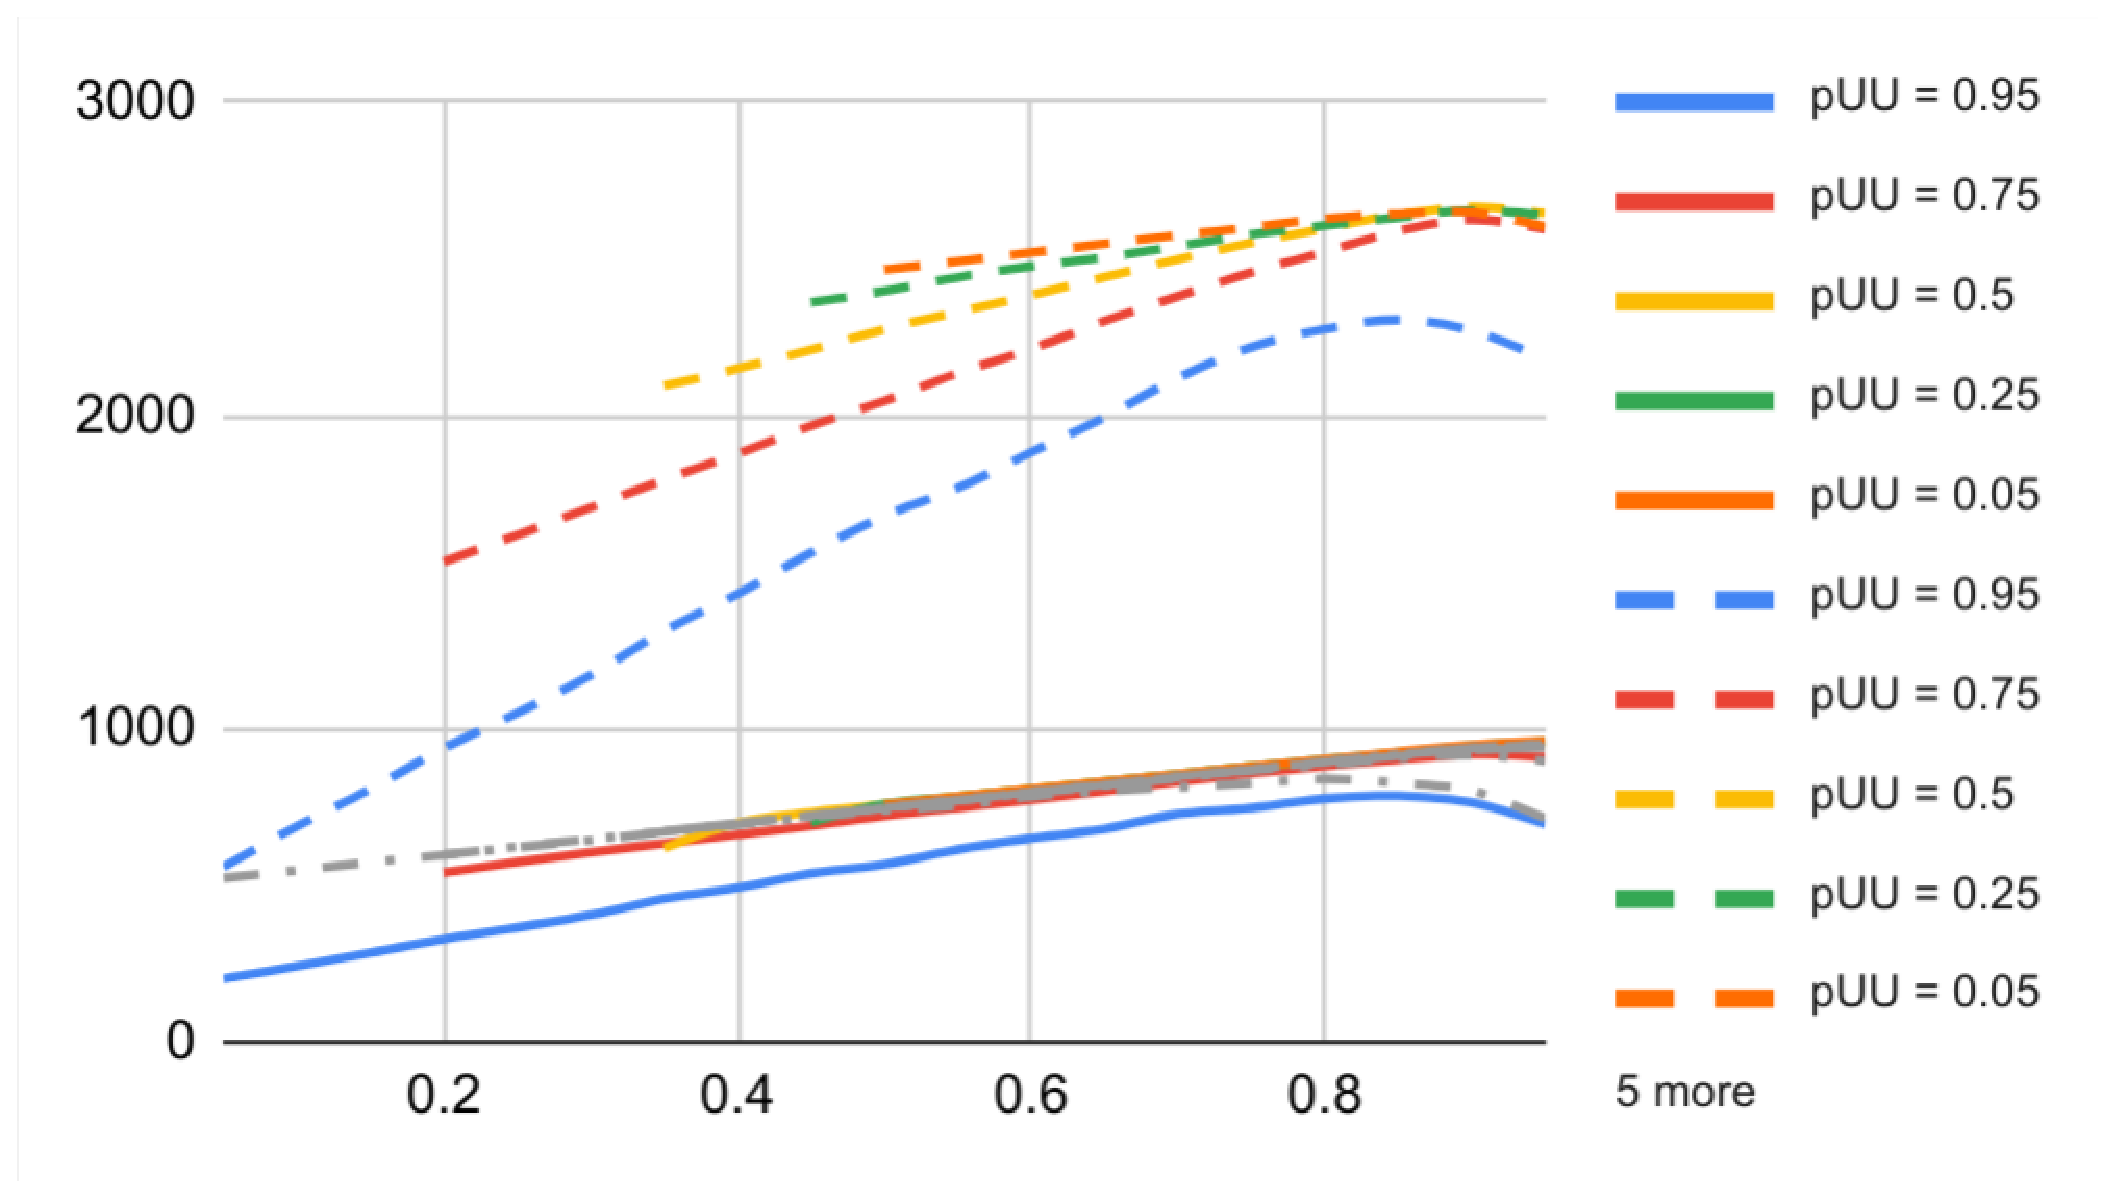
\includegraphics[scale=0.22]{generated_medium}}
  \caption{Delta debugging (dashed) vs brute force (grey), Entropy Debugging (solid) for medium probabilities}
%%\label{fig_example1.ps}
\end{figure}

In the above chart, Entropy Debugging is compared to Delta Debugging and a naive
brute force algorithm for "normal" markov probabilities. The x axis represents
the overall percentage of waste in an input, and the style of the line marks the
algorithm in question (solid = entropy debugging, dashed = Delta Debugging, grey
dash dot = brute force). Each algorithm is plotted for multiple transition
properties (correlation between waste/non-waste in the input): 95\% correlation,
75\% correlation, no correlation (50\%), 75\% discorrelation, 95\%
discorrelation.

For this range of probabilities, Delta Debugging only manages to approach the
performance of the naive solution in the most extreme case of 95\% waste with
95\% correlation. Indeed, Entropy Debugging is only considerably better than the
naive approach in the 95\% correlation plot (and never considerably worse).

This chart clearly does not capture a set of inputs that Delta Debugging was
designed to handle. As probabilities get further and further from these "normal"
(by some definition) probabilities, Delta Debugging gets closer and closer to
Entropy Debugging, with the two meeting when around 99.8\% of an input is waste
with around 99.9\% correlation.

\begin{figure}
  \centerline{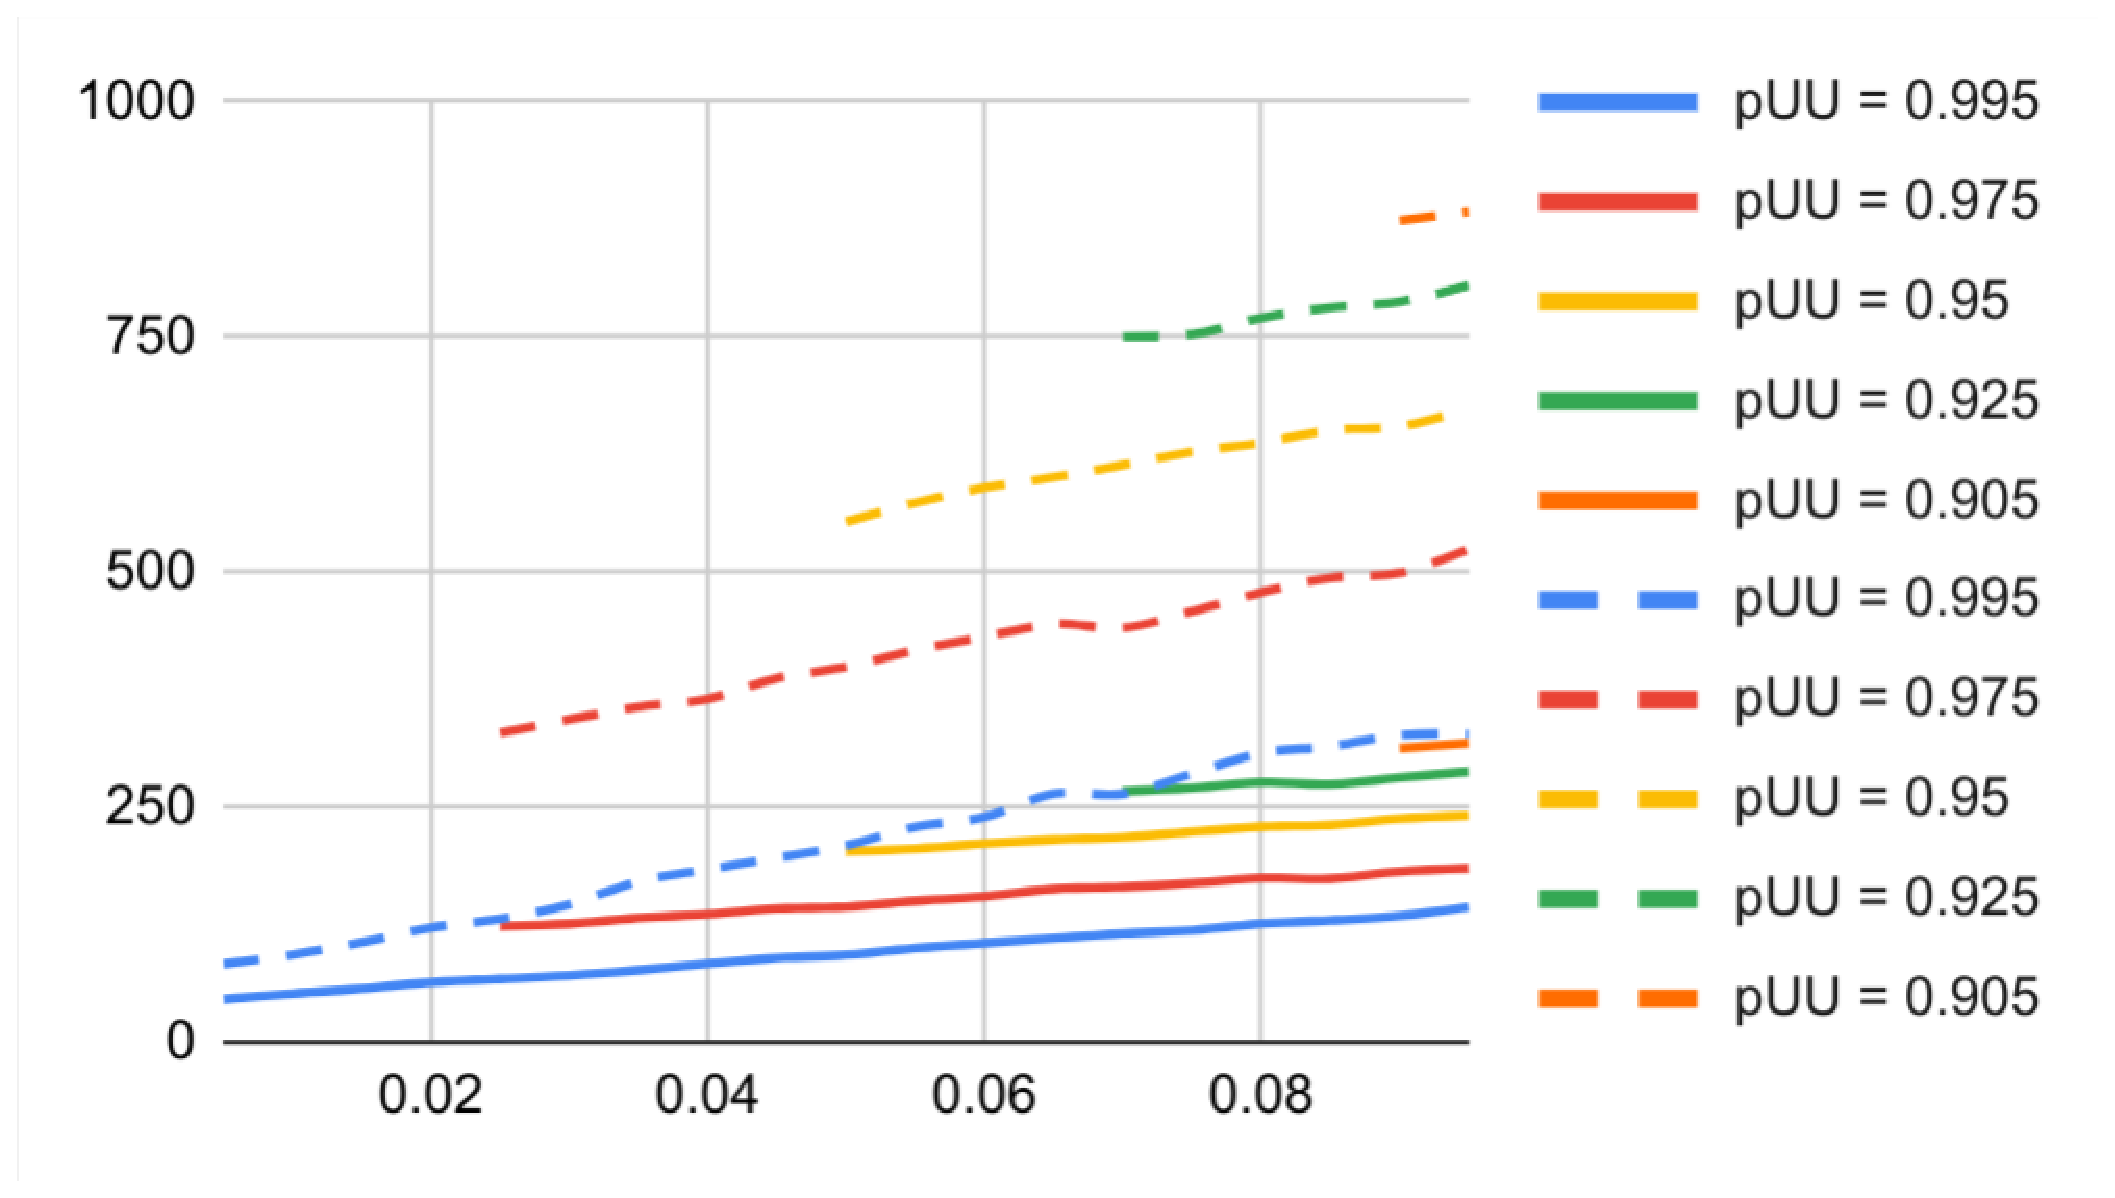
\includegraphics[scale=0.22]{generated_small}}
  \caption{Delta debugging (dashed) vs Entropy Debugging (solid) for small probabilities}
%%\label{fig_example1.ps}
\end{figure}

\begin{figure}
  \centerline{\includegraphics[scale=0.22]{generated_smallest}}
  \caption{Delta debugging (dashed) vs Entropy Debugging (solid) for very small probabilities}
%%\label{fig_example1.ps}
\end{figure}

\subsection{Fuzz Testing Coverage Corpus}

Entropy Debugging was used to minify a fuzz testing corpus while maintaining the
same code coverage.

The fuzzing library Dust is a code coverage guided fuzz testing framework for
Dart. This has been used to generate random Dart programs that may crash the
Dart analyzer. To do so, a corpus of interesting programs is maintained such
that those interesting programs each exercise some unique code path of the fuzz
target.

For the Dart language, there are hundreds of test files that cover most of the
language specification. This is therefore an ideal starting place to find this
set of interesting Dart programs. However, the corpus contains a lot of
redundancy from the perspective of any given fuzz target. The goal is to
therefore quickly minimize this corpus, a task that in theory should be a good
fit for either Delta Debugging or Entropy Debugging.

Here are four example simplifications, charted by input size to runs required by
the two algorithms. In the case of entropy debugging, it has been split out by
time required to simplify vs minimize the input.

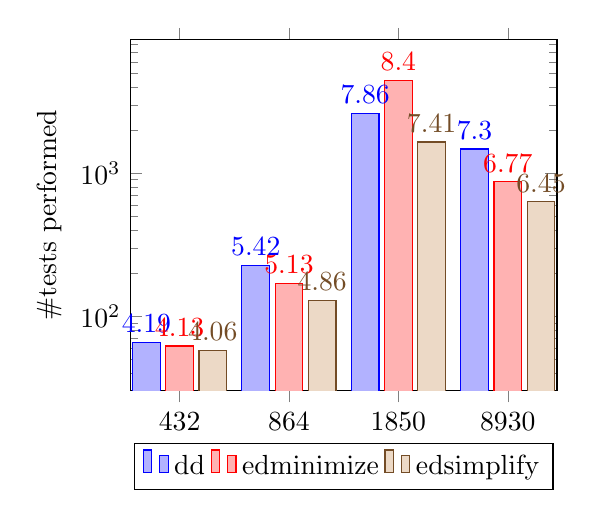
\begin{tikzpicture}
\begin{axis}[
    ybar,
    enlargelimits=0.15,
    legend style={at={(0.5,-0.15)},
      anchor=north,legend columns=-1},
    ylabel={\#tests performed},
    symbolic x coords={432,864,1850,8930},
    xtick=data,
    ymode=log,
    nodes near coords,
    nodes near coords align={vertical},
    ]
\addplot coordinates {(432,66) (864,227) (1850,2603) (8930,1476)};
\addplot coordinates {(432,62) (864,169) (1850,4463) (8930,869)};
\addplot coordinates {(432,58) (864,129) (1850,1653) (8930,630)};
\legend{dd,edminimize,edsimplify}
\end{axis}
\end{tikzpicture}

And here are the median, average, worst results of the three algorithms over
all samples.

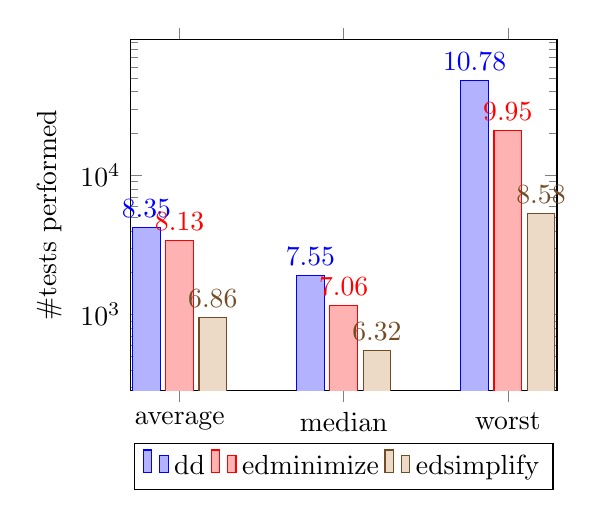
\begin{tikzpicture}
\begin{axis}[
    ybar,
    enlargelimits=0.15,
    legend style={at={(0.5,-0.15)},
      anchor=north,legend columns=-1},
    ylabel={\#tests performed},
    symbolic x coords={average,median,worst},
    xtick=data,
    ymode=log,
    nodes near coords,
    nodes near coords align={vertical},
    ]
\addplot coordinates {(median,1904) (average,4216) (worst,48156)};
\addplot coordinates {(median,1167) (average,3403) (worst,21000)};
\addplot coordinates {(median,557) (average,953) (worst,5330)};
\legend{dd,edminimize,edsimplify}
\end{axis}
\end{tikzpicture}

These data not only show not that Delta Debugging takes 80\% of the time in this
example in the average case, but it also took 43\% of the time in the worst
case.

\subsection{Is miminization useful?}

The previous numbers also raise the question of whether or not
\textit{minimization} is better than \textit{simplification}.

On average, minimization yielded an 11\% smaller input than simplification, even
though it took 3.5x as many tests. For context, the 11\% difference in the
result is a mere 3\% of the input -- and requires 33 additional tests per
additional removed character.

Of course, minimization is still posible with Entropy Debugging, and still
faster in this data set than Delta Debugging (especially in the median and worst
case). However, this paper finds no way to speed up minimization. Under the
statistical and compression theory approach described above, there simply is no
better approach than a character by character search when the entropy of a
sample is high. And at 89\% of the way simplified, that counts as high entropy.
And if a pass at this entropy ends up finding any items in the set that can be
removed, a new pass is required, creating pathological cases in both entropy
debugging as well as delta debugging.

Why is the average only 20\% less for Entropy Debugging even though its median
performance is a 40\% improvemnet from Delta Debugging, which also has the
highest worst case result? This is not a quantitative explanation, but it seems
the answer here is that an inefficient simplification stage leads to a better
minimization stage.

Recall that minimization in this paper specifically refers to Zeller's
definition of 1-minimal\cite{dd}. Stricter minimums can be sought such as
2-minimal and beyond. Anecdotally, it seems that acheiving 1-minimal may
frequently require removing \textit{pairs} or larger chunks of the input, more
in the realm of 2-minimal and beyond. In a character by character sweep, it may
take $n$ passes for some $n$ to acheive 1-minimality.

On the other hand, it seems that Delta Debugging is more likely to have run
additional suboptimal tests in the form of attempting to delete optimistically
large chunks of contiguous characters. These ultimately still result in a
larger average case performance, but they do decrease the likelihood of the
minimization stage taking a large number of passes. (Note that this effect also
does not keep Delta Debugging from claiming the largest recorded worst case
result).

It seems compelling that simplification is a good approximation of 1-minimal
that can be found in significantly less time. Future research to improve
minimization techniques seems prodent, and it seems likely that Delta Debugging
could also benefit from a simplification mode in addition to 1-minimal search.

Similarly, the case studies on mozilla and gcc could be even more drastically
improved if only a \textit{simplified} reproduction were sought instead of a
\textit{minmiized} one.

\subsection{Performance takeaways}

The benchmarking performed lends itself to a selection process between Entropy
Debugging and Delta Debugging.

If a true 1-minimal result is needed, it is possible that entropy-debugging will
not lead to significantly improved results without some improvement over the
process of minimization. However, it still appears to be the better algorithm in
the average and worst case.

If the input is likely close to simplified, Entropy Debugging will yield very
large improvements in performance over Delta Debugging.

If the input is small (approaching ~30 entries) and also far from the minimal
result, Delta Debugging may yield better results due to Entropy Debugging's
limitation of presampling (though this can be tuned).

If the input is very very far from the minimal result (less than 1\% of the
input, is expected to be part of the minimal result), then Delta Debugging may
yield better results due to Delta Debugging's more aggressive approach. This
may also be tunable as a hyperparameter of Entropy Debugging.

This paper proposes that in all other cases, Entropy Debugging seems to
outperform Delta Debugging in all other cases.

This paper also proposes that if a true \textit{minimal} result is \textit{not}
needed, that a simplification from the Entropy Debugging is a much more
efficient approximation.

\subsection{Optimality analysis}

To do: analyze how close entropy debugging gets to the lower bound of
algorithmic performance.

\subsection{Future Work}

There is a large body of future work to be explored in addition to this paper's
findings.

Entropy Debugging currently uses markov models as the only statistical
understanding of the simplification stream's information. This limits the
peformance of Entropy Debugging on inputs that could be described better by
better statistical models, such as machine learning models. While more advanced
models generally require more data, and data collection is itself throttled in
Entropy Debugging, it is possible that new statistical models could lead to
performance improvements, especially in simplifying large corpora of inputs.

Approaches to unify Entropy Debugging with hierarchical approaches such as
HDD\cite{hdd} could yield even larger efficiency. One possibility of such a
unification is to integrate the hierarchical nature of data into the statistical
models of Entropy Debugging rather than changing the overall structure of the
algorithm itself.

Delta Debugging is also capable of comparing minimum failing inputs with maximum
succeeding inputs. While Yu et. al. found that these isolated changes are
typically failure-irrelevant in practical usage\cite{ddRealPerspectives}, work
could be done to find these inputs as part of Entropy Debugging as well for
applications where it may be useful.

An algorithm remains to be found that can efficiently build an optimal runnable
identity encoding, or in general, an optimal ordered probabilistic tree. Doing
so may have implications for Decision Tree Learning in general, and would also
improve the performance of Entropy Debugging.

More advanced compression techniques than huffman code exists. Indeed, it is the
simplicity of huffman codes that make them easily applicable to this particular
simplification problem. However, it is possible that these more advanced
compression techniques such as Arithmetic Coding and ANS could be adapted to
produce runnable identity codes that could be used by Entropy Debugging.


%%%
%%%In order to get started in generating a two-column version of your paper, please format the document with 0.75in top margin, 1.5in bottom margin and 0.825in left and right margins.  Break the text into two sections one for the title heading, and another for the body of the paper.  
%%%
%%%The format of the heading is not critical, on the other hand formatting of the body of the text is the primary goal of this exercise.  This will allow you to see that the figures are matched to the column width and font size of the paper.  The double column of the heading section is set to 1.85in for the first column, a 0.5in spacing, and 4.5in for the second column.  For the body of the paper, set it to 3.34in for both columns with 0.17in spacing, both are right justified. 
%%%
%%%The information that is the focus of this exercise is found in 
%%%section~\ref{sect_figure}.
%%%Please use this template to format your paper in a way that is similar to the printed form of the Journal of Mechanical Design.  This will allow you to verify that the size and resolution of your figures match the page layout of the journal.  The ASME Journal of Mechanical Design will no longer publish papers that have the errors demonstrated here.
%%%
%%%ASME simply requires that the font should be the appropriate size and not be blurred or pixilated, and that lines should be the appropriate weight and have minimal, preferably no, pixilation or rasterization.
%%%
%%%The journal uses 10pt Times Roman Bold for headings, but Times Bold is good enough for this effort.  The text is set at 9pt Times Roman, and again Times will be fine.  Insert a new line after the heading, and two lines after each section.  This is not exactly right but it is close enough.
%%%
%%%
%%%%%%%%%%%%%%%%%%%%%%%%%%%%%%%%%%%%%%%%%%%%%%%%%%%%%%%%%%%%%%%%%%%%%%%%%
%%%\section{Very Very Very Very Very Very Very Very Very Very Very Long Heading}
%%%
%%%The heading is boldface with upper and lower case letters. 
%%%If the heading should run into more than one line, the run-over is not left-flushed.
%%%
%%%%%%%%%%%%%%%%%%%%%%%%%%%%%%%%%%%%%%%%%%%%%%%%%%%%%%%%%%%%%%%%%%%%%%%%%
%%%\subsection{Second-Level Heading}
%%%
%%%The next level of heading is also boldface with upper and lower case letters. 
%%%The heading is flushed left with the left margin. The spacing to the next heading is two line spaces.
%%%
%%%%%%%%%%%%%%%%%%%%%%%%%%%%%%%%%%%%%%%%%%%%%%%%%%%%%%%%%%%%%%%%%%%%%%%%%
%%%\subsubsection{Third-Level Heading.}
%%%
%%%The third-level of heading follows the style of the second-level heading.
%%%
%%%
%%%%%%%%%%%%%%%%%%%%%%%%%%%%%%%%%%%%%%%%%%%%%%%%%%%%%%%%%%%%%%%%%%%%%%%%%
%%%\section{Use of SI Units}
%%%
%%%An ASME paper should use SI units.  When preference is given to SI units, the U.S. customary units may be given in parentheses or omitted. When U.S. customary units are given preference, the SI equivalent {\em shall} be provided in parentheses or in a supplementary table. 
%%%
%%%%%%%%%%%%%%%%%%%%%%%%%%%%%%%%%%%%%%%%%%%%%%%%%%%%%%%%%%%%%%%%%%%%%%%%%
%%%\section{Footnotes\protect\footnotemark}
%%%\footnotetext{Examine the input file, asme2ej.tex, to see how a footnote is given in a head.}
%%%
%%%Footnotes are referenced with superscript numerals and are numbered consecutively from 1 to the end of the paper\footnote{Avoid footnotes if at all possible.}. Footnotes should appear at the bottom of the column in which they are referenced.
%%%
%%%
%%%%%%%%%%%%%%%%%%%%%%%%%%%%%%%%%%%%%%%%%%%%%%%%%%%%%%%%%%%%%%%%%%%%%%%%%
%%%\section{Mathematics}
%%%
%%%Equations should be numbered consecutively beginning with (1) to the end of the paper, including any appendices.  The number should be enclosed in parentheses and set flush right in the column on the same line as the equation.  An extra line of space should be left above and below a displayed equation or formula. \LaTeX\ can automatically keep track of equation numbers in the paper and format almost any equation imaginable. An example is shown in Eqn.~(\ref{eq_ASME}). The number of a referenced equation in the text should be preceded by Eqn.\ unless the reference starts a sentence in which case Eqn.\ should be expanded to Equation.
%%%
%%%\begin{equation}
%%%f(t) = \int_{0_+}^t F(t) dt + \frac{d g(t)}{d t}
%%%\label{eq_ASME}
%%%\end{equation}
%%%
%%%%%%%%%%%%%%%%%%%%%%%%%%%%%%%%%%%%%%%%%%%%%%%%%%%%%%%%%%%%%%%%%%%%%%%%%
%%%\section{Figures}
%%%\label{sect_figure}
%%%
%%%All figures should be positioned at the top of the page where possible.  All figures should be numbered consecutively and centered under the figure as shown in Fig.~\ref{figure_ASME}. All text within the figure should be no smaller than 7~pt. There should be a minimum two line spaces between figures and text. The number of a referenced figure or table in the text should be preceded by Fig.\ or Tab.\ respectively unless the reference starts a sentence in which case Fig.\ or Tab.\ should be expanded to Figure or Table.
%%%
%%%
%%%%%%%%%%%%%%%%%%%%%%%%%%%%%%%%%%%%%%%%%%%%%%%%%%%%%%%%%%%%%%%%%%%%%%%%%
%%%%%%%%%%%%%%%%%%% begin figure %%%%%%%%%%%%%%%%%%%
%%%\begin{figure}[t]
%%%\begin{center}
%%%\setlength{\unitlength}{0.012500in}%
%%%\begin{picture}(115,35)(255,545)
%%%\thicklines
%%%\put(255,545){\framebox(115,35){}}
%%%\put(275,560){Beautiful Figure}
%%%\end{picture}
%%%\end{center}
%%%\caption{The caption of a single sentence does not have period at the end}
%%%\label{figure_ASME} 
%%%\end{figure}
%%%%%%%%%%%%%%%%%%% end figure %%%%%%%%%%%%%%%%%%% 
%%%%%%%%%%%%%%%%%%%%%%%%%%%%%%%%%%%%%%%%%%%%%%%%%%%%%%%%%%%%%%%%%%%%%%%%%
%%%
%%%In the following subsections, I have inserted figures that have been provided by authors in order to demonstrate what to avoid.  In each case the authors provided figures that are 3.25in wide and 600dpi in the .tif graphics format.  The papers containing these figures have been held from production due to their poor quality. 
%%%
%%%%%%%%%%%%%%%%%%%%%%%%%%%%%%%%%%%%%%%%%%%%%%%%%%%%%%%%%%%%%%%%%%%%%%%%%
%%%\subsection{The 1st Example of Bad Figure}
%%%
%%%%%%%%%%%%%%%%%%% begin figure %%%%%%%%%%%%%%%%%%%
%%%%%% 3.34in is the maximum width you can have for a figure
%%%\begin{figure} 
%%%\centerline{\psfig{figure=figure/FMANU_MD_05_1107_11.ps,width=3.34in}}
%%%\caption{Example taken from a paper that was held from production because the image quality is poor.  ASME sets figures captions in 8pt, Helvetica Bold.}
%%%\label{fig_example1.ps}
%%%\end{figure}
%%%%%%%%%%%%%%%%%%% end figure %%%%%%%%%%%%%%%%%%%
%%%
%%%In order to place the figure in this template using MSWord, select ����Insert Picture from File,���� and use wrapping that is  ����top and bottom.����  Make sure the figure is 3.25in wide.
%%% 
%%%Figure~`\ref{fig_example1.ps}
%%%was taken from a recent paper that was held from publication, because the text is fuzzy and unreadable.  It was probably obtained by taking a screen shot of the computer output of the author����s software.  This means the original figure was 72dpi (dots per inch) on a computer screen.  There is no way to improve the quality such a low resolution figure.
%%% 
%%%In order to understand how poor the quality of this figure is, please zoom in slightly, say to 200\%.  Notice that while the font of the paper is clear at this size, the font in the figures is fuzzy and blurred.  It is impossible to make out the small symbol beside the numbers along the abscissa of the graph.  Now consider the labels ����Time���� and ����Cost.����  They are clearly in fonts larger that the text of the article, yet the pixilation or rasterization, associated with low resolution is obvious. This figure must be regenerated at higher resolution to ensure quality presentation.
%%%
%%%The poor quality of this figure is immediately obvious on the printed page, and reduces the impact of the research contribution of the paper, and in fact detracts from the perceived quality of the journal itself.
%%%
%%%
%%%
%%%%%%%%%%%%%%%%%%%%%%%%%%%%%%%%%%%%%%%%%%%%%%%%%%%%%%%%%%%%%%%%%%%%%%%%%
%%%\subsection{The 2nd Example of Bad Figure}
%%%
%%%%%%%%%%%%%%%%%%% begin figure %%%%%%%%%%%%%%%%%%%
%%%\begin{figure} 
%%%\centerline{\psfig{figure=figure/FMANU_MD_05_1272_5.ps,width=3.34in}}
%%%\caption{While this figures is easily readable at a double column width of 6.5in, when it is shrunk to 3.25in column width the text is unreadable.   This paper was held from production.}
%%%\label{fig_example2.ps}
%%%\end{figure}
%%%%%%%%%%%%%%%%%%% end figure %%%%%%%%%%%%%%%%%%%
%%%
%%%Figure~\ref{fig_example2.ps}
%%%demonstrates a common problem that arises when a figure is scaled down fit a single column width of 3.25in.  The original figure had labels that were readable at full size, but become unreadable when scaled to half size.  This figure also suffers from poor resolution as is seen in the jagged lines the ovals that form the chain.
%%%
%%%This problem can be addressed by increasing the size of the figure to a double column width of 6.5in, so the text is readable.  But this will not improve the line pixilation, and a large low resolution figure is less desirable than a small one.  This also significantly expands the length of the paper, and may cause it to exceed the JMD nine page limit.  Additional pages require page charges of \$200 per page.  It is best to regenerate the figure at the resolution that ensures a quality presentation.
%%%
%%%
%%%%%%%%%%%%%%%%%%%%%%%%%%%%%%%%%%%%%%%%%%%%%%%%%%%%%%%%%%%%%%%%%%%%%%%%%
%%%\subsection{The 3rd Example of Bad Figure}
%%%%%%%%%%%%%%%%%%% begin figure %%%%%%%%%%%%%%%%%%%
%%%\begin{figure} 
%%%%\centerline{\psfig{figure=figure/FMANU_MD_04_1274_13.ps,width=3.34in}}
%%%\centerline{\psfig{figure=figure/FMANU_MD_04_1274_13.ps,width=3.25in}}
%%%\caption{Another example of a figure with unreadable text.  Even when the paper was expanded to double column width the text as shown in Fig.~\ref{fig_example4.ps} was of such low quality that the paper was held from production.}
%%%\label{fig_example3.ps}
%%%\end{figure}
%%%%%%%%%%%%%%%%%%% end figure %%%%%%%%%%%%%%%%%%%
%%%
%%%%%%%%%%%%%%%%%%% begin figure %%%%%%%%%%%%%%%%%%%
%%%%%% the maximum width in double column is 6.85in
%%%\begin{figure*} 
%%%\centerline{\psfig{figure=figure/FMANU_MD_04_1274_13.ps,width=6.85in}}
%%%\caption{A figure expanded to double column width the text from Figure~\ref{fig_example3.ps}}
%%%\label{fig_example4.ps}
%%%\end{figure*}
%%%%%%%%%%%%%%%%%%% end figure %%%%%%%%%%%%%%%%%%%
%%%An author provided the high resolution image 
%%%in Fig.~\ref{fig_example3.ps}
%%%that was sized to a single column width of 3.25in.  Upon seeing the poor quality of the text, the publisher scaled the image to double column width as shown in Fig.~\ref{fig_example4.ps} 
%%%at which point it took half of a page.  The publisher went on to do this for all eight figures generating four pages of figures that the author did not expect. ASME stopped production of the paper even with the larger figures due to the pixilation of the font.
%%%
%%%Clearly the text in this figure is unreadable, and it is doubtful that the author can print the output in a way that it is readable.  This is a problem that the author must solve, not the publisher. 
%%%
%%%As you might expect, I have many more examples, but in the end the author is the best judge of what is needed in each figure.  ASME simply requires that the image meet a minimum standard for font and line quality, specifically the font should be the appropriate size and not be blurred or pixilated, and that lines should be the appropriate weight and have minimal, preferably no, pixilation or rasterization.
%%%
%%%
%%%%%%%%%%%%%%%%%%%%%%%%%%%%%%%%%%%%%%%%%%%%%%%%%%%%%%%%%%%%%%%%%%%%%%%%%
%%%\section{Tables}
%%%
%%%%%%%%%%%%%%%%%%%%%%%%%%%%%%%%%%%%%%%%%%%%%%%%%%%%%%%%%%%%%%%%%%%%%%%%%
%%%%%%%%%%%%%%%%%% begin table   %%%%%%%%%%%%%%%%%%%%%%%%%%
%%%\begin{table}[t]
%%%\caption{Figure and table captions do not end with a period}
%%%\begin{center}
%%%\label{table_ASME}
%%%\begin{tabular}{c l l}
%%%& & \\ % put some space after the caption
%%%\hline
%%%Example & Time & Cost \\
%%%\hline
%%%1 & 12.5 & \$1,000 \\
%%%2 & 24 & \$2,000 \\
%%%\hline
%%%\end{tabular}
%%%\end{center}
%%%\end{table}
%%%%%%%%%%%%%%%%%%% end table %%%%%%%%%%%%%%%%%%% 
%%%%%%%%%%%%%%%%%%%%%%%%%%%%%%%%%%%%%%%%%%%%%%%%%%%%%%%%%%%%%%%%%%%%%%%%%
%%%
%%%All tables should be numbered consecutively  and centered above the table as shown in Table~\ref{table_ASME}. The body of the table should be no smaller than 7 pt.  There should be a minimum two line spaces between tables and text.
%%%
%%%
%%%%%%%%%%%%%%%%%%%%%%%%%%%%%%%%%%%%%%%%%%%%%%%%%%%%%%%%%%%%%%%%%%%%%%%%%
%%%\section{Citing References}
%%%
%%%%%%%%%%%%%%%%%%%%%%%%%%%%%%%%%%%%%%%%%%%%%%%%%%%%%%%%%%%%%%%%%%%%%%%%%
%%%The ASME reference format is defined in the authors kit provided by the ASME.  The format is:
%%%
%%%\begin{quotation}
%%%{\em Text Citation}. Within the text, references should be cited in  numerical order according to their order of appearance.  The numbered reference citation should be enclosed in brackets.
%%%\end{quotation}
%%%
%%%The references must appear in the paper in the order that they were cited.  In addition, multiple citations (3 or more in the same brackets) must appear as a `` [1-3]''.  A complete definition of the ASME reference format can be found in the  ASME manual \cite{asmemanual}.
%%%
%%%The bibliography style required by the ASME is unsorted with entries appearing in the order in which the citations appear. If that were the only specification, the standard {\sc Bib}\TeX\ unsrt bibliography style could be used. Unfortunately, the bibliography style required by the ASME has additional requirements (last name followed by first name, periodical volume in boldface, periodical number inside parentheses, etc.) that are not part of the unsrt style. Therefore, to get ASME bibliography formatting, you must use the \verb+asmems4.bst+ bibliography style file with {\sc Bib}\TeX. This file is not part of the standard BibTeX distribution so you'll need to place the file someplace where LaTeX can find it (one possibility is in the same location as the file being typeset).
%%%
%%%With \LaTeX/{\sc Bib}\TeX, \LaTeX\ uses the citation format set by the class file and writes the citation information into the .aux file associated with the \LaTeX\ source. {\sc Bib}\TeX\ reads the .aux file and matches the citations to the entries in the bibliographic data base file specified in the \LaTeX\ source file by the \verb+\bibliography+ command. {\sc Bib}\TeX\ then writes the bibliography in accordance with the rules in the bibliography .bst style file to a .bbl file which \LaTeX\ merges with the source text.  A good description of the use of {\sc Bib}\TeX\ can be found in \cite{latex, goosens} (see how two references are handled?).  The following is an example of how three or more references \cite{latex, asmemanual,  goosens} show up using the \verb+asmems4.bst+ bibliography style file in conjunction with the \verb+asme2ej.cls+ class file. Here are some more \cite{art, blt, ibk, icn, ips, mts, mis, pro, pts, trt, upd} which can be used to describe almost any sort of reference.
%%%
%%%%%%%%%%%%%%%%%%%%%%%%%%%%%%%%%%%%%%%%%%%%%%%%%%%%%%%%%%%%%%%%%%%%%%%%%
\section{Conclusions}
Conclusions TBD
%%%
%%%This gives you the opportunity to ensure that the figures are sized appropriately, in particular that the labels are readable and match the size of the text in the journal, and that the line weights and resolutions have no pixilation or rasterization.  Poor quality figures are immediately obvious on the printed page, and this detracts from the perceived quality of the journal.
%%%
%%%I am pleased to provide advice on how to improve any figure, but this effort must start with a two-column version of the manuscript. Thank you in advance for your patience with this effort, it will ensure quality presentation of your research contributions.
%%%
%%%
%%%
%%%%%%%%%%%%%%%%%%%%%%%%%%%%%%%%%%%%%%%%%%%%%%%%%%%%%%%%%%%%%%%%%%%%%%%%%
\section{Discussions}
Discussion TBD
%%%More specifically, the following features are not ASME format compliant.
%%%\begin{enumerate}
%%%\item
%%%The format for the title, author, and abstract in the cover page.
%%%\item
%%%The font for title should be 24 pt Helvetica bold.
%%%\end{enumerate}
%%%
%%%\noindent
%%%If you can help to fix these problems, please send us an updated template.
%%%If you know there is any other non-compliant item, please let us know.
%%%We will add it to the above list.
%%%With your help, we shall make this template 
%%%compliant to the ASME journal paper format.
%%%
%%%
%%%%%%%%%%%%%%%%%%%%%%%%%%%%%%%%%%%%%%%%%%%%%%%%%%%%%%%%%%%%%%%%%%%%%%%%%
\begin{acknowledgment}
Acknowledgement TBD
\end{acknowledgment}

%%%%%%%%%%%%%%%%%%%%%%%%%%%%%%%%%%%%%%%%%%%%%%%%%%%%%%%%%%%%%%%%%%%%%%
% The bibliography is stored in an external database file
% in the BibTeX format (file_name.bib).  The bibliography is
% created by the following command and it will appear in this
% position in the document. You may, of course, create your
% own bibliography by using thebibliography environment as in
%
% \begin{thebibliography}{12}
% ...
% \bibitem{itemreference} D. E. Knudsen.
% {\em 1966 World Bnus Almanac.}
% {Permafrost Press, Novosibirsk.}
% ...
% \end{thebibliography}

% Here's where you specify the bibliography style file.
% The full file name for the bibliography style file 
% used for an ASME paper is asmems4.bst.
\bibliographystyle{asmems4}

% Here's where you specify the bibliography database file.
% The full file name of the bibliography database for this
% article is asme2e.bib. The name for your database is up
% to you.
\bibliography{entropy-debugging}
%%%
%%%%%%%%%%%%%%%%%%%%%%%%%%%%%%%%%%%%%%%%%%%%%%%%%%%%%%%%%%%%%%%%%%%%%%%%%
%%%\appendix       %%% starting appendix
%%%\section*{Appendix A: Head of First Appendix}
%%%Avoid Appendices if possible.
%%%
%%%%%%%%%%%%%%%%%%%%%%%%%%%%%%%%%%%%%%%%%%%%%%%%%%%%%%%%%%%%%%%%%%%%%%%%%
%%%\section*{Appendix B: Head of Second Appendix}
%%%\subsection*{Subsection head in appendix}
%%%The equation counter is not reset in an appendix and the numbers will
%%%follow one continual sequence from the beginning of the article to the very end as shown in the following example.
%%%\begin{equation}
%%%a = b + c.
%%%\end{equation}

\end{document}
